%!TEX root = ../thesis.tex

\section{Basics}
\label{sec:basics}

This chapter will lay the theoretical foundation to the work of this thesis and will embed it into the context of current research. The title of this Master's Thesis is:

\vspace{-1em}
\begin{center}
\textbf{
	\titleFirst $~$ --\\ [0.2 cm]
	\titleSecond \\
	\titleThird
}
\end{center}

Introduction of the parts of the title, broken down into its pieces, from back to front

\subsection{System} % (fold)
\label{sub:system}

A \emph{system} is an organized structure containing \emph{elements} or \emph{components} that are directly or indirectly related to and interconnected with each other. The elements and their relations form the whole of the structure. The surrounding of the system is its \emph{environment}.

There is an \emph{internal state} at any point of the system's existence. This state only changes when it gets influenced by stimuli of its environment. A system has \emph{emergent properties} that characterize it. These properties are independent from properties of the element of the system, e.g. water is liquid at room temperature, but the elements it consists of, hydrogen and oxygen, are a gas. Each system is both part of a larger system and can be decomposed into subsystems. Therefore, systems form a hierarchy.

A system has defined spatial and temporal boundaries. There are two types: \emph{open systems} allow exchange of energy or information with their environment, whereas \emph{close systems} naturally do not interact with and are not influenced by its environment. However, also closed systems have interfaces with which it is possible to interact with them, giving input to or receiving output from a system. The mathematical function $f(x) = x^2$ is a system, whereas $x$ is the input (e.g. $-3$), and $f(x)$ is the output ($9$). Based on the black box principle it is not visible how the output gets created, because the inner working of a closed system can not be seen through the interface
\cite{system}.

A practical example for a system is the welfare state: The citizens and the treasury are the main elements. They interact with each other in a way that all citizens pay taxes and the needy citizens receive welfare (healthcare, education, childcare, etc.). The system is open in a sense that through migration, birth or death citizens can come into or leave the system.

\begin{figure}[ht]
  \centering
  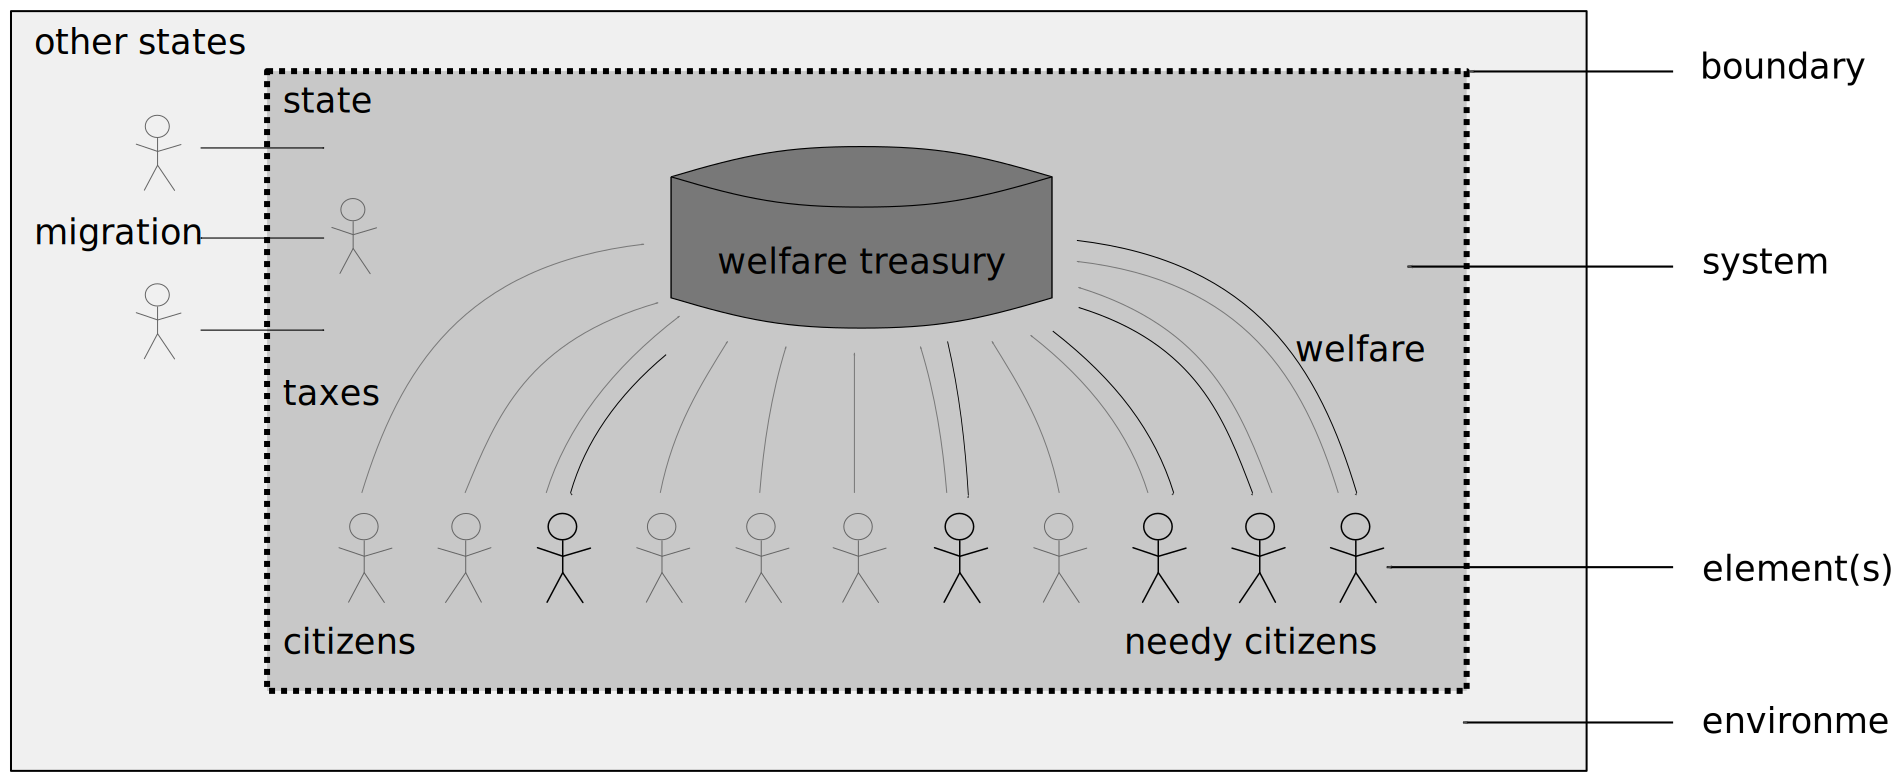
\includegraphics[width = 0.8\textwidth]{graphics/basics/social_system}
  \caption{The welfare state as an example of a system}
  \label{fig:social_system}
\end{figure}


% subsection system (end)


\subsection{Information System} % (fold)
\label{sub:information_system}

An \emph{information system} (IS) is an application that is dealing with the collection, management, analysis and presentation of information. A digital IS is the unity of all its components and their interaction with each other.

\subsubsection{\emph{Information}} % (fold)
\label{ssub:definition_of_information}
The terms ``signs'', ``data'', ``information'' and ``knowledge'' are sometimes used interchangeably and there is no coherent definition for any of them. However, all describe different concepts. This explanation seen in figure \ref{fig:information} is based on the work of \cite{datinfwis}.

\begin{figure}[ht]
    \begin{center}
        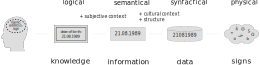
\includegraphics[width=0.4\textwidth]{graphics/basics/information}
    \end{center}
    \caption{signs, data, information and knowledge}
    \label{fig:information}
\end{figure}

There are uncountably infinitely many different \emph{signs} in the world. A sign is the physical representation of something in the real world. Since the real world is continuous, literally anything can be seen as a sign. \emph{Data} is a subset of all possible signs and create the syntactical level of what an information system deals with. Data itself does not have any meaning, but as soon as it is organized, it becomes \emph{information}. However, information is sensitive to its cultural context. The word ~\texttt{Gurkensalat}~ is useful and understandable for anybody who understands the German language and it is therefore an information for him or her. However, for all other people on Earth this is just a random string of letters without any meaning, and therefore no information -- though it is the same data. If information is visualized to and understood by a human and it can be integrated into his or her larger subjective context, it is \emph{knowledge} \cite{nake}. The goal of a visualization is to present as much information as possible in a way that it can be transformed into knowledge by the user.
% subsubsection definition_of_information (end)


\subsubsection{Components} % (fold)
\label{ssub:components_is}

% subsubsection components (end)

The components of an IS can be classified by their task: The \emph{collection} or \emph{acquisition} part describes everything that is related to data input. Data is physically stored and logically managed in a \emph{database} of an information system. The data will be analyzed regarding different aspects of the task in order to make sense of them, transform them into information that can be used to answer the question of the user. The resulting information will be presented in a diagram, a table, a map or any other textual or graphical way on the screen or another output medium of the information system.
\cite{informationSystem}.
All components will be explained in more detail in section %\ref{ssub:gis_components}.

Another possible classification is by hardware, software and data. \emph{Hardware} is the unity of all physical parts of a computer, e.g. the central processing unit, the storage or the graphics card. All electronic devices involved in input, processing or output of information are the system's hardware. On the contrary, \emph{software} provides the functionality and is a set of instructions that controls the hardware and the data in an information system. Software is the component with which humans can interact with the information system through a user interface. The components communicate with each other by exchanging information.

% subsubsection components_is (end)


\subsubsection{Types} % (fold)
\label{ssub:types}

Information systems can be further classified by their type or usage scenario. The main distinction based on the level of separation between data and application: In a \emph{Desktop IS}, all elements are stored on the end user's device and using the syste normally requires installation of software. A distributed \emph{Web IS}, consists of a remote server side, on which the storage and management of the actual data happens, and the client side on which the user communicates with the system. It hosts the user interface that is rendered in a Web browser.

% subsubsection types (end)

% subsection information_system (end)


\subsection{Geographic Information System} % (fold)
\label{sub:geographic_information_system}

If the majority of the information in a system has a spatial relation to the Earth, its surface, its lithosphere, atmosphere or the social or economical structure of its habitation, it is a \emph{geographic information system} (GIS). There are mainly four components: The idea is that Geodata is put into the system, managed in a geographical database, analyzed regarding different information needs of the user to present as information on a digital map -- the output of the system (figure \ref{fig:gis_components}).

\begin{figure}[ht]
  \centering
  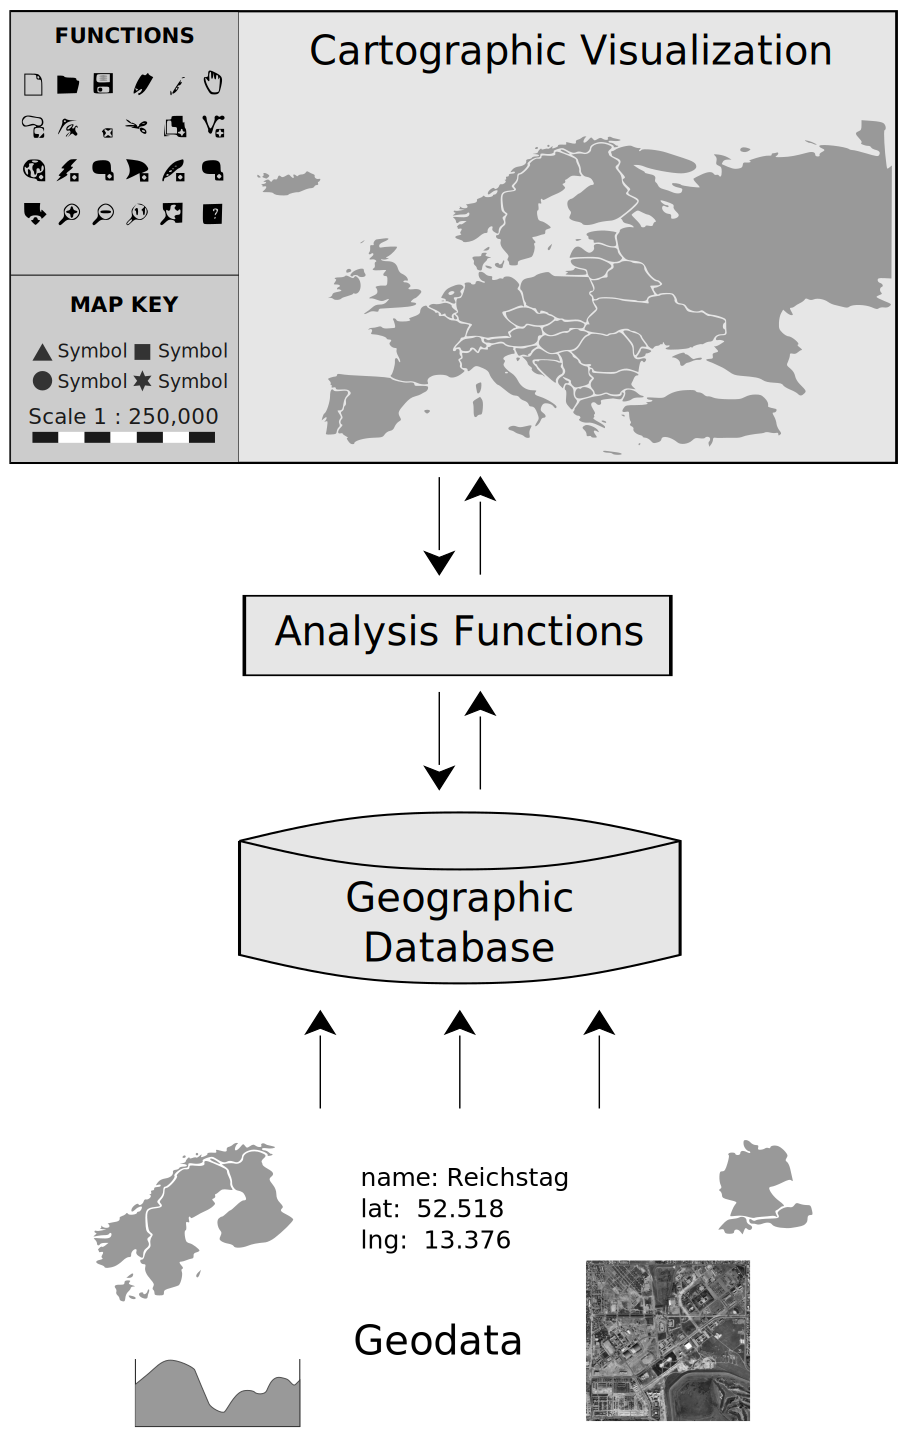
\includegraphics[width=0.48\textwidth]{graphics/basics/gis_components}
  \caption{Main components of a GIS}
  \label{fig:gis_components}
\end{figure}

GIS are important tools for geographers to solve problems in their research field. But also people for in their in everyday lives they are helpful, e.g. to get directions on the fastest way from A to B
\cite{ngGeography}.


\subsubsection{\emph{Geography}} % (fold)
%\label{ssub:geography}

The term ``geography'' comes from Greek ~\emph{\textgamma\textepsilon\textomega\textgamma\textrho\textalpha\textphi\textiota\textalpha / geographia}~, literally ``describing the earth''
\footnote{
  \textit{Geography},
  Dictionary.com, based on Random House Dictionary, 2015,
  URL: \url{http://dictionary.reference.com/browse/geography},
  last access: 23.10.2015
}.
It is a science that studies the interplay between the landscapes and environments of the Earth on the one hand and the people, their cultures, societies and economies on the other. Therefore, geography can be divided into physical geography, a natural science, and human geography, a social science -- making it an interdisciplinary field
\cite{rgsGeography}.

Research in geography aims to understand where things are found, why they are there and how they developed over time. In regional geography, another subbranch, also the causes of social or environmental differences between cultures and landscapes want to be found. Geography focuses on the interconnectivity between all elements of physical and human geography, which gets expressed in Tobler's First Law of Geography: ``Everything is related to everything else, but near things are more related than distant things.''
\footnote{
  ``A computer movie simulating urban growth in the Detroit region'',
  Waldo Tobler, 1970
  Economic Geography, 46(2): 234-240.
}

Geographers use different technology and techniques to analyze geographic processes and to answer their research questions. The oldest and most important among those are maps. A map is a graphical expression of something that is not tangible: a part of the real world. A map shows the physical, environmental, political, economical or social properties of the Earth in order for the user of the map to get the most relevant information for his task, may it be orientation, learning or teaching. The ``art and science of making maps'' is the field of \emph{cartography}
\footnote{
  \textit{History of maps and cartography},
  James S. Aber,
  URL: \url{http://academic.emporia.edu/aberjame/map/h_map/h_map.htm},
  last access: 24.10.2015
}. Since maps sample the real world, they have a natural constraint: ``No map can perfectly replicate the real world, since it inevitably generalizes, abstracts and approximates the complexity of the reality''
\cite[p. 181]{knowles2008placing}

% TODO:                 had? had? has had? is having?
The scientific background of GIS is \emph{geographic information science} (GISci) that studies patterns in natural and human development, e.g. erosion of valleys, literacy rate, natural hazards and deals with approaches and techniques to manage, analyze and visualize this information
\cite{ngGeography}.

% subsubsection geography (end)


\subsubsection{Model of the Earth} % (fold)
\label{ssub:model_of_the_earth}

A GIS deals with \emph{geo-objects}, a piece of \emph{geospatial data} representing an object from the real world, e.g. a country, a city or a lighthouse. The system needs to unambiguously locate each object on, underneath or close to the Earth's surface by \emph{geographic coordinates}. They allow to locate an object directly in the coordinate system of the geodetic datum. In order to do that, a geo-object has to be expressed in the coordinate system of the Earth. Therefore the shape of the Earth has to be analyzed and and then modeled in a way that can be represented in an information system. This model is called the \emph{geodetic datum}, it needs to be necessarily accurate on the one hand and reasonably abstract on the other hand.


\paragraph{The shape of the Earth} % (fold)
\label{par:the_shape_of_the_earth}

Our planet is a large object in the solar system. In reality, the Earth's shape, measured by scientists in the field of \emph{geodesy}, is rather complicated. In the Babylonian Empire ($\approx$ 2000-539 BC) the theory of the Earth being a flat disc surrounded by an infinite body of water
%(a theory still valid in some southern parts of the United States of America)
evolved. It was not until measurements by the Greek scientists Pythagoras and Aristotle (340 BC) that this theory was rejected. They proved the earth to be a three-dimensional spherical object. It took almost 2000 years until Sir Isaac Newton (1687) reasoned that due to the centrifugal forces of the rotating Earth the shape has to flattened at the poles and is therefore better described as an \emph{ellipsoid} with two radii: the polar radius and the slightly larger equatorial radius
\cite[pp. 69-77]{bolstad2008gis}.

\begin{figure}[ht]
  \centering
  \includegraphics[width = 0.3\textwidth]{graphics/basics/ellipsoid}
  \caption{The ellipsoidal model}
  \small{based on \cite[Fig. 3-3, p. 72]{bolstad2008gis}}
  \label{fig:ellipsoid}
\end{figure}

However, the ellipsoidal model disregards the fact that the surface of the Earth is not flat but rather consists of both deep oceanic trenches and high mountains. Therefore the gravitational field of the Earth is not homogeneous either: the actual \emph{mean sea level} surface, the reference for the height of mountains or buildings, varies from 106 meter below to 85 meter above the uniform sea level of the ellipsoid model. These discoveries in the \nth{20} century led to the complex \emph{geoid} model (see figure \ref{fig:geoid}). Sir George Gabriel Stokes in 1849 was a pioneer in this field, the latest and most accurate measurements for the shape of the Earth are the result of the GOCE satellite launched in March 2009
\cite{geoid, geoidESRI}.

%TODO: if too much time, a graphic about the history of the shape pf the Earth would be nice :-)

\begin{figure}[ht]
  \centering
  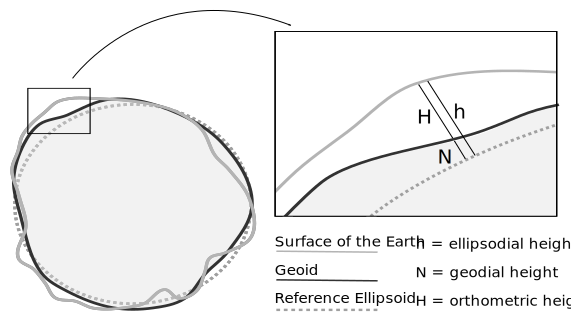
\includegraphics[width=0.66\textwidth]{graphics/basics/geoid}
  \caption{The geoid model, differences are very exaggerated}
  \small{based on \cite[Fig. 3-6, p. 75]{bolstad2008gis}}
  \label{fig:geoid}
\end{figure}

% paragraph the_shape_of_the_earth (end)

\paragraph{Geographic coordinate system} % (fold)
\label{par:geographic_coordinate_system}

The reference ellipsoid is the basis for the model that is used to determine an object's position relative to the Earth's surface. On the surface, there are two dimensions: The \emph{longitude} (\texttt{x}) in east-to-west direction and he \emph{latitude} (\texttt{y}) varying in north and south. Lines of constant latitude are running horizontally and are called \emph{parallels}, lines of constant longitude are \emph{meridians} appearing in vertical direction. Additionally, there is \emph{elevation} (\texttt{z}) as the third dimension identifying the height, i.e. the distance to mean sea level. In this thesis only \texttt{x} and \texttt{y} are covered.

All parallels are circles with their center on the axis between the poles. They are all parallel to each other, no two parallels intersect. The longest parallel is the \emph{Equator} splitting the world into the northern and the southern hemisphere.
%Each latitude in the northern hemisphere has exactly one counterpart in the southern hemisphere with the same size and the same distance to the Equator.
All meridians are semicircles running from the North to the South Pole and with their center in the center of the Earth. Therefore all meridians have the same length, they only differ in a third point on the circle along the equator. The \emph{Prime Meridian} is running through Greenwich, a suburb on London.

The ellipsoidal model of the Earth is represented in a \emph{spherical coordinate system}. A position of a point in a 3D coordinate system determines its distance to the origin, in this case the Earth's center. Each point can be unambiguously defined by three values
(see Figure \ref{fig:geo-coordinates}):

\begin{enumerate}
  \item The rotation angle along the Equator, defining its longitude: $\gamma = [-180\degree ~...~ +180\degree]$ \\
  with the Prime Meridian being $0\degree$ longitude
  \item The rotation angle along the Prime Meridian, defining its latitude: $\phi = [-90\degree ~...~ +90\degree]$ \\
  with the Equator being $0\degree$ latitude
  \item The distance to the origin: $r \in \mathbb{N}_0$ \hfill
  \cite[pp. 26-28]{bolstad2008gis}
\end{enumerate}

\begin{figure}[ht]
  \centering
  \includegraphics[width=0.8\textwidth]{graphics/basics/geo-coordinates}
  \caption{Geo-coordinates using latitude and longitude}
  \label{fig:geo-coordinates}
\end{figure}


% paragraph geographic_coordinate_system (end)

% subsection spatial_reference (end)

\paragraph{Geodetic datum} % (fold)
\label{par:geodetic_datum}


One main task of a GIS is to accurately visualize the Earth on a map. Since the Earth is an inhomogeneous three-dimensional shape but the output medium is a two-dimensional computer screen or piece of paper, it has to be transformed. First the Earth has to be modeled using the \emph{geodetic datum}. It consists of two parts: The approximation of the Earth's surface in a the Cartesian coordinate system with the origin and a set of reference points used to accurately locate a point.

Geodetic datums can be very accurate in one region of the world, i.e. the model fits the real geoid very well, but inaccurate in another region. This is the main reason why there are a lot of different geodetic datums used in the world. The same coordinates in two different geodetic datums define two different points on Earth. In order to be accurate is essential to know the geodetic datum of the coordinates
\cite[p. 80]{bolstad2008gis}.

The \emph{World Geodetic System 1984 (WGS84)} is a model that found worldwide acceptance and is used in all major Web-based mapping services like \emph{OpenStreetMap} and is implemented in the GPS unit of all major smart phones.

% paragraph geodetic_datum (end)

% subsubsection model_of_the_earth (end)


\subsubsection{Map Projections} % (fold)
\label{ssub:map_projections}

Based on the geodetic datum a three-dimensional representation of the Earth in form of a globe would be a possible medium to view the planet. When seen perpendicular onto the world, a globe represents sizes, shapes, distances and directions of objects close to the viewpoint with a reasonable accuracy. However, they are very space-consuming and cumbersome. For a precise measurement of distances, following a route or examining a terrain model, the globe would have to be very large. Therefore, the desired medium for practical purposes is a two-dimensional map.

The basic problem to be solved is that the Earth is a spherical object, its surface is curved and it is therefore not straightforward to project it onto a flat 2D map. The meridians which are lines of equal value converge at the poles. Neighboring meridians (distance: 1\degree) have a distance of 111 km at the Equator and 0 km at the poles. They do not form a right-angled grid with the parallels and therefore no Cartesian coordinate system. This is the reason why the geometries of the spherical Earth will be distorted when displayed on a flat 2D Cartesian coordinate system. \cite[p.79]{bolstad2008gis}

% \begin{figure}[ht]
%   \centering
%   \includegraphics[width=0.66\textwidth]{graphics/basics/distortion}
%   \caption{Distortion visualized by circles on a 2D map as a Cartesian coordinate system}
%   (on the 3D Earth all circles have the same size)
%   \label{fig:distortion}
% \end{figure}

There are two main classifications of map projections: The \emph{projection family} with respect to the geometric shape used for the transformation: \emph{cylindrical}, \emph{conical} and \emph{azimuthal} or \emph{planar projection}). Secondly, the \emph{distortion characteristics} with respect to the map property that is preserved. There are \emph{equivalent}, \emph{conformal}, \emph{equidistant}, \emph{zenithal} and compromise projections. Most families and characteristics can be mixed, e.g. it is possible to create a cylindrical, a conical and an azimuthal equivalent map projection
\cite{mapProjectionKrygier}.


\paragraph{Projection Families} % (fold)
\label{subp:projection_families}

The basis of geometrical map projections are \emph{developable surfaces} onto which the ellipsoidal model of the Earth is projected. The are mainly three geometric shapes that are used as reference surfaces: cylinders, cones and planes. The model is fitted in or on the surface touching it in at least one point or line. The idea is that there is a projection source from which rays are shot through the ellipsoid on the surface, projecting each point of the ellipsoid onto the surface (as seen in figure \ref{fig:projections}). This principle is known from the ray casting technique in computer graphics
\cite{mapProjectionGeokov}.

\begin{figure}[ht]
  \centering
  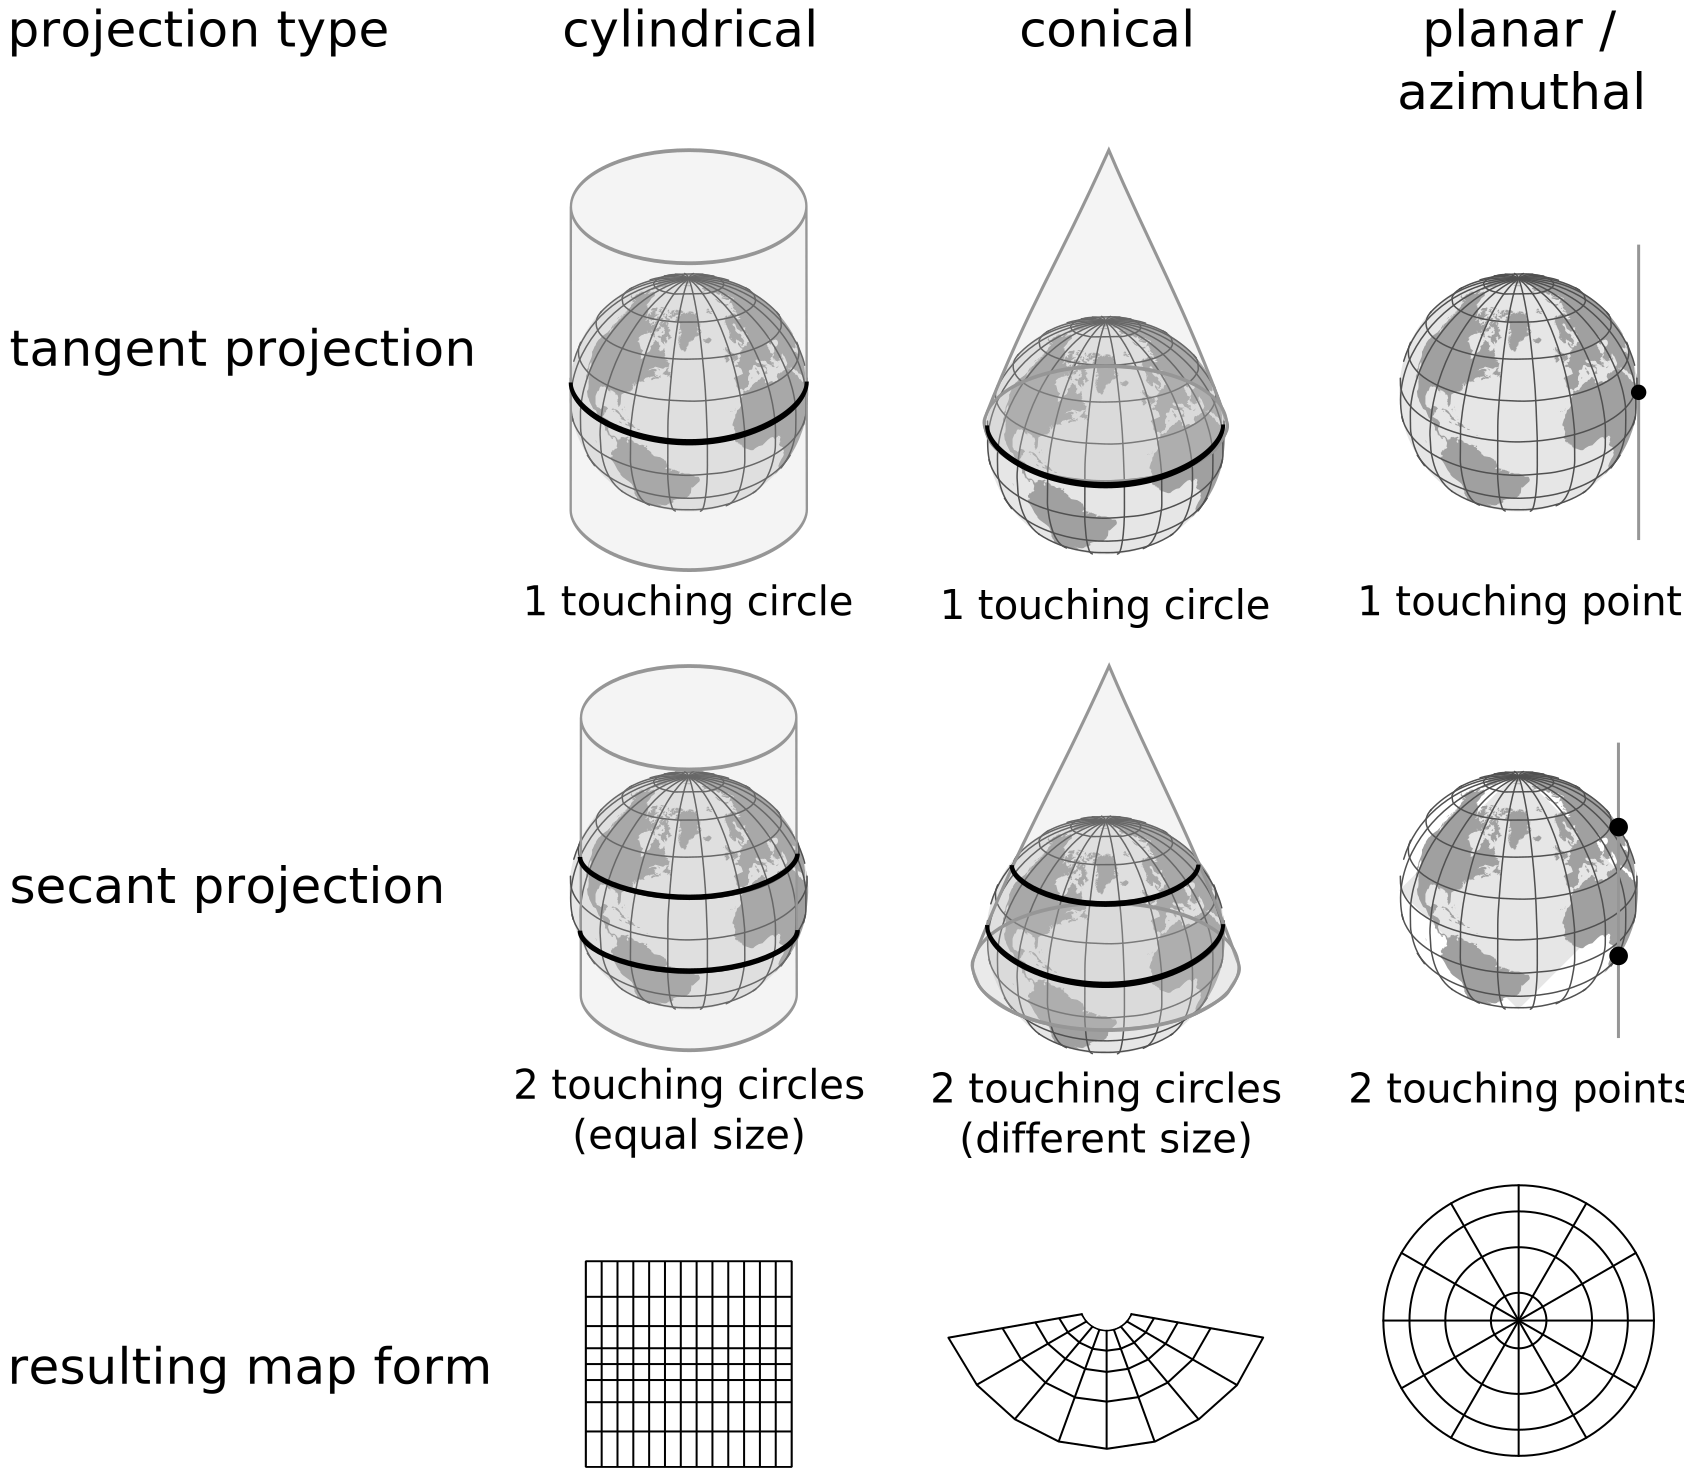
\includegraphics[width=0.73\textwidth]{graphics/basics/projections}
  \caption{Three different developable surfaces for map projections \protect\footnotemark}
  \label{fig:projections}
\end{figure}

\footnotetext{
  based on: \textit{Coordinate Reference Systems},
  QGis Documentation,
  URL: \url{http://docs.qgis.org/2.0/en/docs/gentle_gis_introduction/coordinate_reference_systems.html},
  last access: 27.10.2015
}

In praxis, also pure mathematical map projections are used, e.g. pseudocylindrical, sinusoidal or Mollweise projections. They are much more complex and have the goal to reduce the overall distortion
\cite[p.99]{bolstad2008gis}.

% subsubsection projection_families (end)


\paragraph{Distortion characteristics} % (fold)
\label{par:distortion_characteristics}

To flatten a spherical surface onto a flat surface, transformations such as stretching, tearing or shearing have to be performed. % affine? non-affine?
A map projection is only accurate at the \emph{standard lines}, i.e. the point(s) or line(s) where the developable surface touches or intersects the ellipsoid. In all other parts the map will in some ways be deformed. That causes distortion in at least one of the following properties of a map: shape (angle), size (area),  direction or distance of features on the map. There is no perfect map projection. Each projection can preserve maximum two of these properties at a cost of distorting the others. The cartographer has to make a compromise and choose a set of characteristics that are important while accepting a distortion in the other properties.

\emph{Tissot's indicatrices} visualize the distortion patterns in the form of ellipses on the map. Their size, shape and orientation are caused by the map projection and show the distortion at this point of the map. Using indicatrices the advantages and disadvantages of each map projection can be shown.

There are two mutual exclusive characteristics: \emph{equivalent} and \emph{conformal}. Equivalent projections preserve the sizes and areas of features on the map, whereas conformal projections preserves angles and the shapes of objects. Every map projection that is area-preserving distorts shapes at the same time, and vice versa
\cite{mapProjectionGeokov}.

\begin{figure}[ht]
  \centering
  \begin{subfigure}{0.59\textwidth}
    \centering
    \includegraphics[width=0.9\linewidth]{graphics/basics/projection_distortion_lambert.png}
    \caption{Lambert cylindrical projection \protect\footnotemark}
  \end{subfigure}
  \begin{subfigure}{0.39\textwidth}
    \centering
    \includegraphics[width=0.9\linewidth]{graphics/basics/projection_distortion_mercator.png}
    \caption{Mercator cylindrical projection \protect\footnotemark}
  \end{subfigure}
  \caption{Comparison of equivalent and conformal map projections}
  \label{fig:lambert_vs_mercator}
\end{figure}

% reset footnotecounter by 1 (for left subfigure caption)
\addtocounter{footnote}{-1}
\footnotetext{
  \textit{Tissot indicatrix world map Lambert cyl equal-area proj},
  Eric Gaba / Sting (Wikimedia), June 2008
  URL: \url{https://commons.wikimedia.org/wiki/File:Tissot_indicatrix_world_map_Lambert_cyl_equal-area_proj.svg},
  last access: 28.10.2015
}

% set footnotecounter to next footnote (for right subfigure caption)
\addtocounter{footnote}{1} % count to next footnote
\footnotetext{
  \textit{Tissot indicatrix world map Mercator proj},
  Eric Gaba / Sting (Wikimedia), September 2008
  URL: \url{https://commons.wikimedia.org/wiki/File:Tissot_indicatrix_world_map_Mercator_proj.svg},
  last access: 28.10.2015
}

The \emph{Mercator projection} (figure \ref{fig:lambert_vs_mercator}b) is an angle-preserving map. It was used for nautical navigation because of a very helpful property: constant compass bearing. A straight line on a Mercator map crosses all meridians in the same angle, a so called \emph{loxodrome}. A navigator only has to follow this line and never needs to reset the compass, because it will always point in the same direction. This is not the shortest way from A to B, but the easiest to navigate. The disadvantage of Mercator maps are the large area distortions towards the poles, which can be seen at the sizes of the ellipses. The best example visualizing the problem is Greenland: On the map it seems almost as large as Africa, whereas in reality Africa is 14 times larger than Greenland.
\cite{mapProjectionGeokov}

This scale becomes obvious in the area-preserving \emph{Lambert projection} (figure \ref{fig:lambert_vs_mercator}a). Tissot's indicatrices all have the same size, but their shapes get distorted towards the poles. This map shows the real size of Africa, but largely distorts the shape of Europe. However, for thematic mapping and teaching purposes equivalent projections are well-suited, because they accurately show the areas of the countries.
\cite{mapProjectionGeokov}

The result of an \emph{equidistant} projection is a map that in relation to the scale accurately shows the distances between certain points on the map.

\vspace{0.5em} % unfortunately necessary to prevent awkward linebreak in footnotes
\begin{figure}[ht]
  \centering
  \begin{subfigure}{0.62\textwidth}
    \centering
    \includegraphics[width=0.9\linewidth]{graphics/basics/projection_distortion_equirectangular.png}
    \caption{Equirectangular equidistant cylindrical projection \protect\footnotemark}
  \end{subfigure}
  \begin{subfigure}{0.37\textwidth}
    \centering
    \includegraphics[width=0.9\linewidth]{graphics/basics/un_logo}
    \caption{Logo of the United Nations \protect\footnotemark}
  \end{subfigure}
  \caption{Two examples of equidistant map projections}
  \label{fig:equidistant_projections}
\end{figure}

% reset footnotecounter by 1 (for left subfigure caption)
\addtocounter{footnote}{-1}
\footnotetext{
  \textit{Tissot indicatrix world map equirectangular proj},
  Eric Gaba / Sting (Wikimedia), June 2008
  URL: \url{https://commons.wikimedia.org/wiki/File:Tissot_indicatrix_world_map_equirectangular_proj.svg},
  last access: 28.10.2015
}

% set footnotecounter to next footnote (for right subfigure caption)
\addtocounter{footnote}{1} % count to next footnote
\footnotetext{
  \textit{Logo of the United Nations},
  Shizhao (Wikimedia), 13.06.2007
  URL: \url{https://commons.wikimedia.org/wiki/File:Logo_of_the_United_Nations_(B\%26W).svg},
  last access: 28.10.2015,
  Comment: This work is excerpted from an official document of the United Nations prior to 17. September 1987.
}

% pidgeon
% irc.freenode.net#slab

Figure \ref{fig:equidistant_projections}b shows a prominent example: The Unites Nations chose a map for their logo from which all points on the map have the correct distance to the North Pole. The equirectangular projection in Figure \ref{fig:equidistant_projections}a has a slightly different property: any meridian is true to scale and therefore all distances along the meridians are accurate. However, the ellipses on the map are distorted in both shape and size, so the map is neither conformal nor equivalent. Air navigation charts or seismology make use of the equidistant property e.g. to show distances from major cities to the epicenter of an earthquake.
\cite{mapProjectionGeokov}

\emph{Zenithal} or \emph{azimuthal} projections preserve directions from the center point to all other points on the map (see figure \ref{fig:zenithal_projection}). It is only possible in the family of planar projections and can be combined with a conformal, equivalent and equidistant property. These maps are used whenever directional relationships are important, for example in navigational charts.

\begin{figure}[ht]
  \centering
  \includegraphics[width=0.3\textwidth]{graphics/basics/projection_distortion_azimuthal.png}
  \caption{Lambert azimuthal (zenithal) equivalent projection \protect\footnotemark}
  \label{fig:zenithal_projection}
\end{figure}

\footnotetext{
  \textit{Lambert azimuthal equal-area projection SW},
  Strebe (Wikimedia), 15. August 2011
  URL: \url{https://commons.wikimedia.org/wiki/File:Lambert_azimuthal_equal-area_projection_SW.jpg},
  last access: 28.10.2015
}

If no characteristic is explicitly important but the overall distortion shall be minimized, a \emph{compromise projection} can be used. They do not preserve any property, but are a trade-off in the distortion of all other properties. The Robinson projection in figure \ref{fig:robinson_projection} is a well-known example. All Tissot's indicatrices not on the Equator are distorted in size, shape and direction, but compared to the Mercator or Lambert projection, the magnitude of distortion is lower.

\begin{figure}[ht]
  \centering
  \includegraphics[width=0.65\textwidth]{graphics/basics/projection_distortion_robinson.png}
  \caption{Robinson projection \protect\footnotemark}
  \label{fig:robinson_projection}
\end{figure}

\footnotetext{
  \textit{Tissot indicatrix world map Robinson},
  Eric Gaba / Sting (Wikimedia), June 2008
  URL: \url{https://commons.wikimedia.org/wiki/File:Tissot_indicatrix_world_map_Robinson_proj.svg},
  last access: 28.10.2015
}

% subsubsection map_projections (end)


\subsubsection{Geographic Data Models} % (fold)
\label{ssub:data_models}

Geo-objects consist of spatial data (\emph{where?}), that allow to locate an object on Earth with geographic coordinates, and attribute data (\emph{what?}) that describe the object, e.g. a name, color, weight or a description. Attribute values can be characterized by their level of measurement (table \ref{tab:data_scale}).

Geographic coordinates are usually recorded either in degree-minutes-second (\texttt{DMS}, e.g. \texttt{50\degree~58' 22''}) or in decimal degree (\texttt{DD}, e.g. \texttt{50.973}) notation
\cite[pp. 30, 79]{bolstad2008gis}.
There are also indices describing a location on Earth using a value that more people can easier deal with. The most common example is an address of a person or the name of a building describing a specific point and a postal code specifying a certain area in a country. These indices and the exact representation of the object's location in coordinates are linked through key registers called \emph{Gazetteers}.


\begin{table}[ht]
\begin{center}
\begin{tabular}{l l l l l}
    \toprule
    Type & Scale & Relationship & Operations & Example \\
    \midrule
    \multirow{2}{*}{categorial} & nominal & none & $A=B$, $A\neq B$ & gender \\
    & ordinal & order / rank & \rotatebox[origin=c]{180}{$\Lsh$} + $A>B$, $A<B$ & exam grade \\
    \midrule
    \multirow{2}{*}{cardinal} & interval & \rotatebox[origin=c]{180}{$\Lsh$} + same distance & \rotatebox[origin=c]{180}{$\Lsh$} + ($A+B$, $A-B$) & date of birth \\
    & ratio & \rotatebox[origin=c]{180}{$\Lsh$} + absolute zero point & \rotatebox[origin=c]{180}{$\Lsh$} + ($A\cdot B$, $A/B$) & age \\
    \bottomrule
\end{tabular}
\caption{Level of measurements}
\small{\cite[p. 31]{bolstad2008gis}}
\label{tab:data_scale}
\end{center}
\end{table}


The real world is infinitely large and continuous. Even just the relevant geographical features, like forests, streets, houses, cities or country borders are infinite in detail. But storage in a computer system is finite. In order to model these continuous phenomena in a GIS, a relevant subset of them has be sampled to create discrete spatial data. It can be represented in two ways: in a \emph{raster} or in a \emph{vector} model.

\begin{figure}[ht]
  \centering
  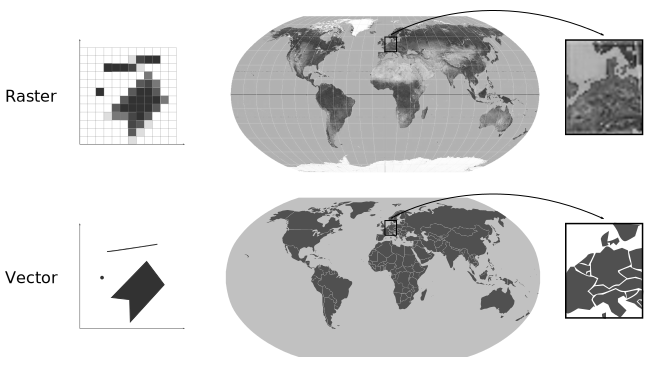
\includegraphics[width=0.9\textwidth]{graphics/basics/raster_vector}
  \caption{Comparison of the raster and the vector model}
  \label{fig:raster_vector}
\end{figure}


\paragraph{Raster model} % (fold)
\label{par:raster_model}

Raster graphics are well known from the working of a computer screen or digital photography: There is a regular grid of \texttt{x} by \texttt{y} pixels and each pixel has a defined color. With an appropriate resolution a high-quality picture with fine details can emerge.

The raster model for spatial data works with the same principle, but a cell does not necessarily have to consist of a color value, but it can also be a value expressing a height, a population density or an elevation. For visualization purposes however this value is often translated into a color value using a certain color scheme. There is a fixed \emph{cell dimension} for the grid.
% Attribute data can be linked to spatial data in a separate table.

The raster model is very simple. It allows straightforward rendering, only affine transformations have to be applied in order to project the raster graphic on the screen. In the same way map layers, an important concept in GIS, are easily achievable: with affine transformations the layers can be projected onto each other. The disadvantage of the raster model is the inflexibility of the regular grid, especially in terms of accuracy: To double the accuracy, the cell dimension has to be halved and therefore the number of cells increased by factor four.

The raster model is useful for data that changes frequently and has fine details or many variations. That applies to cardinal data, e.g. color values in an aerial image, absolute values for distribution of pollution, or the elevation in a hilly area
\cite[pp.42-48]{bolstad2008gis}.
Raster graphics are used by most map engines for the basic map layer in form of map tiles, e.g. in OpenStreetMap or the satellite image of the Earth by NASA in Google Maps (figure \ref{fig:google_maps_satellite}).

\begin{figure}[ht]
  \centering
  \includegraphics[width=0.8\textwidth]{graphics/basics/google_maps_satellite.png}
  \caption{The basic map layer for Google Maps  \protect\footnotemark}
  \label{fig:google_maps_satellite}
\end{figure}

\footnotetext{
  \textit{Google Maps},
  URL: \url{https://www.google.com/maps/@51.2090662,13.2328189,3563505m/data=!3m1!1e3},
  Imagery \textcopyright2015 Landsat, Data SIO, NOAA, U.S. Navy, NGA, GEBCO, IBCAO, U.S. Geological Survey, Map data \textcopyright2015 Google, ORION-ME,
  last access: 29.10.2015
}

% credits to Fr. Bamberg:
% "Der Bau bestimmt die Eigenschaften und
% die Eigenschaften bestimmen die Verwendung"

% paragraph raster_model (end)


\paragraph{Vector model} % (fold)
\label{par:vector_model}

In the vector model, each object is a mathematically described geometric primitive whose exact location is specified by a set of points given in geographic coordinates. Additionally, each object has a unique ID and can be linked with attributes (e.g. color or name) in a separate table. There are three basic geometric primitives (figure \ref{fig:geometric_primitives}):

\begin{figure}[ht]
  \centering
  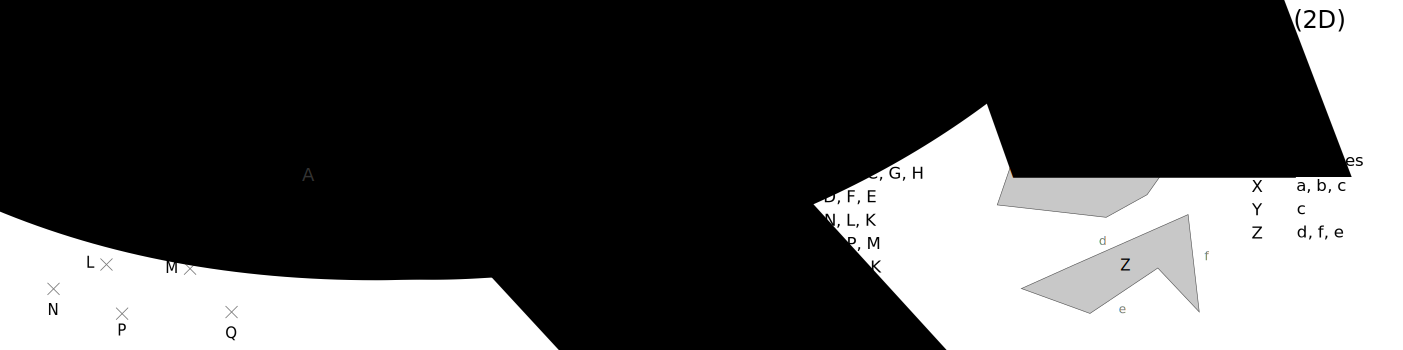
\includegraphics[width=0.8\textwidth]{graphics/basics/geometric_primitives}
  \caption{The basic geometric primitives point, polyline and polygon}
  \label{fig:geometric_primitives}
\end{figure}

\begin{enumerate}
  \item[0D] A \emph{point} is the most fundamental object in vector geometry in a GIS. It has no dimension, no size and is only defined by its position, given in geographic coordinates. One point is independent from all other ones. Points can be used e.g. to represent landmarks or villages.
  \item[1D] A \emph{polyline} is constructed by an ordered set of points with at least one start and one end point. A polyline can have a direction. The model contains only the points, it is up to the program to visualize the segment between the points at run time. While they can be joined with a straight lines they could also be connected with cubic splines to create a smooth Bézier curve. A street can be expressed by a polyline, a one-way street by a directed polyline.
  \item[2D] A \emph{polygon} is again an ordered set of polylines creating a closed area. The first point of the first polyline is also the last point of the last polyline in the set. A polygon can be \emph{simple} with a \emph{concave} or \emph{convex} form, \emph{weakly simple} if it contains holes or \emph{complex}, if there are crossing polylines (see figure \ref{fig:polygon_properties}). Any area, e.g. a lake or a state, can be described by a polygon.
\end{enumerate}

\begin{figure}[ht]
  \centering
  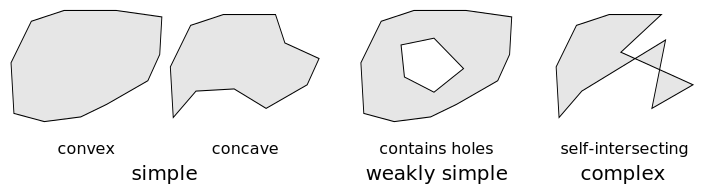
\includegraphics[width=0.8\textwidth]{graphics/basics/polygon_properties}
  \caption{Different properties of polygons}
  \label{fig:polygon_properties}
\end{figure}

Also three-dimensional objects are possible, containing a set of polygons assembling the surface of the volume. Additionally, a \emph{polypolyline} represents multiple separate lines belonging to one logical entity, e.g. an interrupted highway. In the same way, a \emph{polypolygon} describes the union of multiple separate areas, e.g. a set of islands of an archipelago.

The vector model can be extended with a topology, if the geometries are represented in a \emph{topological vector model}. The elements in this topological space are nodes (0D), edges (1D), meshes (2D) and volumes (3D) and they correspond directly to the geometric primitives stated above. An example can be seen in figure \ref{fig:topological_vector_model}. A topology is planar, if all features are on a two-dimensional surface, i.e. there are no overlapping edges without a node at their intersection point. A \emph{topological vector model} has strict connectivity, a ``clean'' geometry, if the topology is planar and each interior edge has exactly two adjacent areas and
each edge contains at least two nodes
\cite[pp.37-39]{bolstad2008gis}.

\begin{figure}[ht]
  \centering
  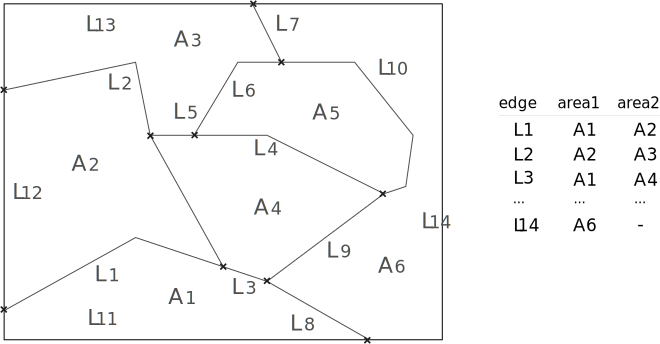
\includegraphics[width=0.7\textwidth]{graphics/basics/topological_vector_model}
  \caption{An example of a topological vector model and an adjacancy table}
  \label{fig:topological_vector_model}
\end{figure}

Scale-independence is one of the biggest advantages of a vector model: Vector graphics always appear sharp. The data model is more compact in comparison to the raster model, especially for larger areas without changes there is less data. The topological vector model has a great asset: if an edge between two adjacent areas changes, the connectivity and adjacency does not change and therefore also the topology stays constant. The lookup for neighboring areas is very fast if the topology ensures strict connectivity: The neighbors of an area can be found in the adjacency table.

One problem of the vector data model is its potential complexity. Since vector data has to be rasterized to be shown on the screen, the computational effort increases with complexity. A solution approach is zoom-depended rendering of the geometry: the smaller the scale factor, the more simplified the geometry will be rendered.
%Another problem appears in the creation of vector data: boundary generalization is important issue, e.g. for sampling a rugged coastline. The world has to be sampled as accurate as possible by leaving out unimportant details.
One more critical aspect is the creation of a clean geometry: it can be cumbersome and require a lot of manual adjustment, for example ensuring strict connectivity by manually connecting nodes
\cite[pp.33-42]{bolstad2008gis}.

Vector models are suitable whenever there the real world can easily be represented with discrete geometric objects, e.g. for streets or park areas. They are used to represent networks, e.g. for example public transport in a city. The most straightforward use of vector models are for the representation of discrete phenomena in real world, e.g. for interior borders of countries, which are straight lines between manually defined border points. Common file types for vector data with spatial reference are the open file formats GeoJSON (\texttt{.geojson})
\footnote{
  \textit{GeoJSON},
  IETF Geographic JSON Working Group,
  URL: \url{http://geojson.org/},
  last access: 30.10.2015
}
and Scalable Vector Graphics (\texttt{.svg})
\footnote{
  \textit{W3C SVG Working Group},
  IETF Geographic JSON Working Group,
  URL: \url{http://www.w3.org/Graphics/SVG/},
  last access: 30.10.2015
}
or ESRI Shapefiles (\texttt{.shp})
\footnote{
  \textit{ESRI Shapefile Technical Description},
  ESRI White Paper, July 1998,
  URL: \url{http://www.esri.com/library/whitepapers/pdfs/shapefile.pdf},
  last access: 30.10.2015
}
, an industry standard.
%TO DO: references

% paragraph vector_model (end)

% subsubsection data_models (end)


\subsubsection{Input} % (fold)
\label{ssub:input}

Spatial Data for a GIS can either be acquired from existing sources or retrieved manually. One of the most exhaustive collections of geographic data in public domain is hosted by Natural Earth
\footnote{
  \textit{Natural Earth},
  URL: \url{http://www.naturalearthdata.com/downloads/},
  last access: 30.10.2015
}.
There is physical data (e.g. coastlines, rivers, or glacier areas) and cultural data (e.g. political borders, cities, roads, airports or timezones). OpenStreetMap also opens its database to the public
\footnote{
  \textit{Planet OSM},
  URL: \url{http://planet.openstreetmap.org/},
  last access: 30.10.2015
}.
Additionally there is free geodata for special purposes, like regions or statistical data for the USA
\footnote{
  \textit{Free GIS Data - GIS Data Depot},
  geocommunity,
  URL: \url{http://data.geocomm.com/catalog/index.html},
  last access: 30.10.2015
}
or terrain models and administrative regions for Germany
\footnote{
  \textit{Dienstleistungszentrum des Bundes für Geoinformation und Geodäsie},
  Geodatenzentrum,
  URL: \url{http://www.geodatenzentrum.de/geodaten},
  last access: 30.10.2015
}.

% subsubsection input (end)


\subsubsection{Management} % (fold)
\label{ssub:management}

A \emph{Database Management System} (DBMS) is a software system for the administration of data, i.e. storage, retrieval, validation of data and their relations. A DBMS has the task to maintain security, performance, stability and allow multi-user access on the same data, following the \emph{client-server} principle.

Data and functions are separated from each other using a \emph{multi-tier architecture} that is best visualized in an example of a Web-based GIS (compare with figure \ref{fig:gis_components}): The Web browser on the client side hosts the map including content and the tools in the user interface. If the user interacts with a tool the client sends a request to the Web server for new data. The processing layer on the server checks the request and forwards it to the DBMS which translates the request into a query to the database. The result will be handed back to the processor that transforms the data into information and sends it to the client. On the map the new information will be shown.

Following this principle multiple clients can independently from each other get new data from the server, but also multiple processing layers for different purposes can simultaneously request data fro the database, ensured by the DBMS. Another advantage of the clear separation between the data (\emph{model}), the user interface (\emph{view}) and the processing layer (\emph{controller}) follows directly from the \emph{model-view-controller pattern}: One part can be changed without interfering the other parts, e.g. if the map interface changes, the data can stay untouched and an implementation of a new database technology has no consequences to the interface.

There are mainly two types of DBMS: the most common \emph{relational} database and \emph{object-relational} databases that are inspired by the features of object-oriented programming paradigms. Pure \emph{object-oriented} databases will not be covered in this section.

\paragraph{Relational databases} % (fold)
\label{par:relational_databases}
Databases are built around logical entities that have a discrete set of attributes associated with them, e.g. a city (entity) has a name, a location, a major, a state it belongs to etc. For each member of the entity there is one value for each attributes (e.g. the name of the city is Weimar) which is of a certain data type (integer, decimal, string, boolean, etc.). Entities is a database are represented in a table with rows (one row per member), columns (one column per attributes) and cells (attribute value for this member). Each entity has one attribute that unambiguously identifies each record in the table, the \emph{primary key}.

In a \emph{Relational Database Management System} (RDBMS), entities can be related to each other by three types of relations:
\begin{enumerate}
  \item If each member of one entity has directly one member from another entity associated, it is a direct attributional relation (\emph{1:1}), e.g. each city has exactly one major.
  \item If each member can have several members of another entity related to it, there is a one-to-many (\emph{1:n}) relationship, e.g. each state can have many cities, but a city can only be in one state.
  \item If multiple members from one entity can be related to multiple members of another entity, it is called many-to-many relation (\emph{m:n}), e.g. each river can flow through several states and each state can have several rivers.
\end{enumerate}
The relations are implemented via their primary keys. Many-to-many relationships require another connection table that uses the primary keys from both entities as \emph{foreign keys} in the new table and links them, e.g. if river \texttt{r} flows through countries \texttt{x} and \emph{y}, the connection table would have one record linking \texttt{r} to \texttt{x} and one linking \texttt{r} to \texttt{y}. The entities and their relations are visualized in an \emph{entity-relationship model} (E-R model), as seen in figure \ref{fig:er_example}.

\begin{figure}[ht]
  \centering
  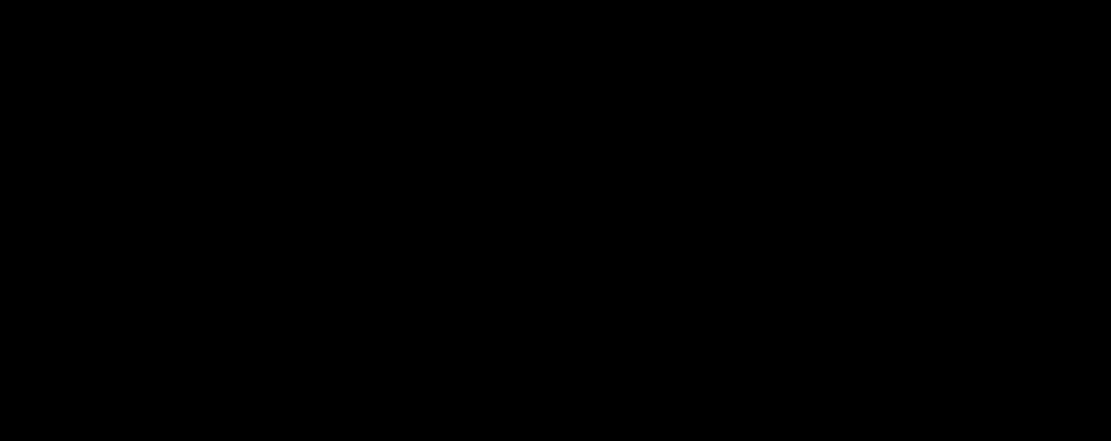
\includegraphics[width=0.75\textwidth]{graphics/basics/er_example}
  \caption{Example for a simple entity-relationship model.}
  \label{fig:er_example}
\end{figure}

Data can be retrieved from a database using the \emph{Structural Query Language} (SQL). An example query to get the names of cities from the state \texttt{Thüringen} in alphabetical order is:
\begin{verbatimtab}
  SELECT     city.id, city.name
  FROM       (city JOIN state ON city.state = state.id)
  WHERE      state.name = ``Thüringen''
  ORDER BY   city.name
\end{verbatimtab}

SQL can also be used to add or manipulate data in a database, e.g. with the \texttt{CREATE} or \texttt{INSERT INTO} commands.

The main goals for each database user is to maintain its correctness,consistency and simplicity and to reduce redundancy in the data. This can be achieved by \emph{normalizing} the database:
\begin{enumerate}
  \item To free the collection of relations from undesirable insertion, update and deletion dependencies.
  \item To reduce the need for restructuring the collection of relations, as new types of data are introduced, and thus increase the life span of application programs.
  \item To make the relational model more informative to users.
  \item To make the collection of relations neutral to the query statistics, where these statistics are liable to change as time goes by.
\footnote{
  \textit{Further Normalization of the Data Base Relational Model},
  E.F. Codd,
  [p. 34]
}
\end{enumerate}

Two examples for RDBMS are \emph{MySQL}, the ``the world's most popular open source database''
\footnote{
  \textit{MySQL :: About MySQL},
  URL: \url{https://www.mysql.com/about/},
  last access: 31.10.2015
}, and the serverless, zero-configuration library \emph{SQLite}
\footnote{
  \textit{SQLite Home Page},
  URL: \url{https://www.sqlite.org/},
  last access: 31.10.2015
}.

% paragraph relational_databases (end)

\paragraph{Object-relational databases} % (fold)
\label{par:object_relational_databases}

Relational databases are well-suited to manage data in simple form without complex database user requirements. However, there can be more difficult queries to the database. Given the example in figure \ref{fig:er_example}, a user would like to know all rivers that are in and close to the state \texttt{Thüringen}, i.e. they smallest distance between the river and the state border is less than 50 km. A query for that request should look like this:
\begin{verbatimtab}
  SELECT    river.name
  FROM      (river JOIN state JOIN state_rivers)
  WHERE     state_rivers.state = state.id AND
            state_rivers.river = river.id AND
            state.name = ``Thüringen'' AND
            distance (state.location, river.location) < 20
  ORDER BY  city.name
\end{verbatimtab}

This query needs to call the function \texttt{distance}, but user-defined functions are not part of SQL. Also, the data type of the attribute \texttt{location} is not simple: it is not a single value, but rather a \texttt{polyline} or a \texttt{polygon}. Complex user-defined data types are also not integrated in SQL.

ORDBMS behave like RDBMS but can handle complex data. For that matter functionality from object-oriented programming are added, so it supports user-defined data types and functions and the principles such as \emph{encapsulation} or \emph{inheritance}.
% scheiße hier... ich habe keinen Bock mehr jeden Mist hier theoretisch zu erklären. Nur darauf eingehen, wenn ich es wirklich später benutze.
%Encapsulation is the ability make the internal state of an object unaccessible to the outside. Whereas it will be possible to get the coordinates of the location of a city with a simple function it will not be possible to change it directly but through a function \texttt{point.} A request for the perimeter of a  of an object and just give the necessary :
One famous example for object-relational databases is \emph{PostgreSQL}, ``the world's most advanced open source database''
\footnote{
  \textit{PostgreSQL: About},
  URL: \url{http://www.postgresql.org/about/},
  last access: 31.10.2015
}.

\paragraph{Spatial databases} % (fold)
\label{par:spatial_databases}
GIS can deal with a lot of coordinate data. This amount of data has to be processed efficiently in order to maintain a good overall system performance. \emph{Spatial databases} are specialized for this matter. They have predefined data types such as \texttt{point}, \texttt{polyline} or \texttt{polygon} and support spatial queries such as functions to solve the point-in-polygon problem or to calculate a distance between two polylines. \emph{PostGIS} is an extension for PostgreSQL that is especially utilized for GIS
\footnote{
  \textit{PostGIS},
  URL: \url{http://postgis.net/},
  last access: 31.10.2015
}.
\emph{SpatiaLite} is a library for the same purpose, extending SQLite's relational database management system
\footnote{
  \textit{SpatiaLite},
  URL: \url{https://www.gaia-gis.it/fossil/libspatialite/index},
  last access: 31.10.2015
}.

% paragraph spatial_databases (end)

% subsubsection management (end)


\subsubsection{Analysis} % (fold)
\label{ssub:analysis}

A GIS shall solve the problem for a user or answer his or her research question. Given a well-filled database with a working DBMS, the data might not answer the research question directly. It has to be sorted, selected or classified in order to convey the required information. For this process there are \emph{spatial operations} on the data in the system. Several operations can be applied in a certain order
\cite[pp. 321-325]{bolstad2008gis}.
Both spatial and attribute data are analyzed to combine the dimensions \emph{where?} and \emph{what?} in order to answer the ultimate question \emph{why?} something is the way it is
\cite[p.xii-xvi]{knowles2002past}.

An example is a system visualizing social developments on Earth. The researcher wants to divide the world into five regions with a similar life expectancy to see if there are spatial discrepancy of advances in global health. He or she has a GIS with all countries and their current life expectancy stored. In order to answer his or her research question, the following steps may be required

\begin{enumerate}
  \item Extract the life expectancy value per country.
  \item Classify the values on a discrete scale from very low to very high and put each country into one of the five classes.
  \item Unify neighboring countries that are in the same class to get five world regions.
  \item Name the five world regions.
  \item Apply a color scheme to the classification and set the background color for each of the five world regions.
  \item Create a legend with the classification and the explanation of the symbols.
  \item Present the resulting map on the screen.
\end{enumerate}

There are special operations for raster data, e.g. spatial interpolation, and for vector data.

Only explain those later that are really important!

graph / network analysis
  what is the shortest way from A to B?
  what is the fastest route from A via B1, B2, ..., Bn nack to A? (TSP)

Polygon geometry
  intersection, (cascaded) Union, (symmetric) difference

Polygon Clipping
  Sutherland-Hodgeman
  Weiler-Atherton

Topology analysis
  test for consistency, connectedness and completeness of topology


% subsubsection analysis (end)

\subsubsection{Presentation} % (fold)
\label{ssub:presentation}

Cartographic visualizations are the interface between the GIS and the human. A map is is the common form. It is a discrete graphical expression of the continuous real world. The creation of a map is not just a scientific, but also a creative process: The form, function and interaction methods shall follow the purpose of the usage of the map.

There is no fixed guideline how to properly design a map, but there are typical elements that are part of every cartographic visualization.The main element is the map itself, using a specific map projection (see section \ref{ssub:map_projections}), a scale and an initial center point. A map is typically structured in a \emph{layer} principle. Each layer is a transparent film showing one specific aspect, e.g. a physical layer showing coastlines, mountains or forests, a political layer showing international borders or a cultural layer showing cities or population densities. The layers are interchangeable, can be switched on and off and serve to serve a different visualization purpose. The map is designed using a certain color scheme, fonts and signatures for all the objects on the map.

Additionally there can be a \emph{title} describing the purpose of the map. A \emph{legend} including the scale bar and north arrow shall explain all symbols used on the map and give orientation. Depending on the degree of interactivity, there can be \emph{menus} with different visualization options, e.g. panning and zooming on the map, switching map layers on and off or changing the color scheme of the map.
\cite[pp. 159-166]{bolstad2008gis}

% example of a good map

The main goal of map design is to give the user nothing but the necessary information he needs to satisfy his or her information need. The cartographer shall use techniques of \emph{cartographic generalization} to minimize information on the map and maximize the knowledge to be extracted from the map. Simplification, smoothing or aggregation help to reduce amount of information. Enlarging, widening or displacement help to focus on the important areas of the map. Selection and classification help the user to get an overview of the information.
\cite{krygier2005making}

Leaflet.js is ``an open-source JavaScript library for mobile-friendly interactive maps''
\footnote{
  \textit{Leaflet - JavaScript library for interactive maps},
  URL: \url{http://leafletjs.com/},
  last access: 02.11.2015
}
that offers functionality to embed a map with a chosen projection in an HTML document, use own map tiles, symbols and markers on the map and tools for zooming and panning.
The same service is provided by \emph{OpenLayers}, a ``A high-performance, feature-packed library for all your mapping needs''
\footnote{
  \textit{OpenLayers 3 - Welcome},
  URL: \url{http://openlayers.org/},
  last access: 02.11.2015
}, just with more features and users.

% subsubsection presentation (end)

% subsubsection components_gis (end)


\subsubsection{Applications} % (fold)
\label{ssub:gis_applications}

GIS are not only for geographers to solve their research problems, but also for the everyday lives of people. Digital maps are used to get directions on the fastest way from A to B, to explore an area and plan holiday trips. But there are other professionals using GIS, e.g. urban planners to analyze the structure of a human settlement and to decide where the next residential area will be placed. Another example is a rescue service operating in inaccessible space: For them it is important to know which areas have already been properly searched by its teams to decide where they should be tasked to next.

% * general purpose complete GIS for private usage
%   open source
%     QuantumGIS  http://www.qgis.org
%     GRASS GIS   http://grass.osgeo.org/
%     SAGA GIS    http://www.saga-gis.org/
%   closed source
%     ArcGIS      https://www.arcgis.com
%     AutoCAD

% Open Geospatial Consortium standards

% * Land information system (cadastral and land-use mapping -> local governments)
% * Environmental information system (environmental programs, disaster management)
% * Network information systems (supplier and disposal management)
% * Specific information systems (tourism, transportation, social service)



% subsection geographic_information_system (end)


\subsection{Historical Geographic Information System} % (fold)
\label{sub:historical_geographic_information_system}

\emph{Historical} or \emph{temporal geographic information systems} (HGIS) combine elements of history and geography into one information system to be able to answer research questions for both historians and geographers: ``situating history in its geographical context and using geographic information to illuminate the past.''
\cite[p. 3]{knowles2008placing}
This manifests the interdisciplinary nature of HGIS and making it also an interesting technology in the context of \emph{digital humanities}, the intersection between humanities and computing. The main distinction to classical GIS is the integration of the component of time, making the system four-dimensional. HGIS collect, manage, analyze and present spatio-temporal information and models changes over time and space
\cite[p. xii]{knowles2002past}.


\subsubsection{\emph{History}} % (fold)
%\label{ssub:history}

History is ``an ideal field for thinking long and hard about important questions''
\cite{ahaFiveCs}.
The Greek word \emph{\textIota\textsigma\texttau\textomikron\textrho\textiota\textalpha / historia}, meaning ``finding out, learning through research, narration of what is learned'', is the origin
\footnote{
  \textit{History},
  Dictionary.com, based on Random House Dictionary, 2015,
  URL: \url{http://dictionary.reference.com/browse/history},
  last access: 23.10.2015
}
and it already signifies the two main modern usage form of the term: To research about and learning something and to tell a story.

There are many different definitions of the word
\emph{history}
\footnote{
  \textit{History},
  Merriam Webster -- an Encyclopædia Britannica Company,
  URL: \url{http://www.merriam-webster.com/dictionary/history},
  last access: 23.10.2015
}. The main goal of history is to study processes in the past to understand the situation in the present and make reasonable decisions for the future. The American Historical Association has developed the ``five C`s of historical thinking [, that] together describe the shared foundations of [the] discipline''\cite{ahaFiveCs}:
\vspace{-1em}
\begin{description}[labelindent=1.5em] % manipulation of indentation
    \item[Change over time]
    The lives of people, their languages and their cultures are continuously changing. Describing these historical changes, triggered by historical events happed in the past, is a major goal of history. Snapshots in the form of historical maps or historical photography are used to tackle this task.
    \item[Context]
    is an important element of historical thinking. The goal is to travel back in time to the moment of event and recreate the world based on primary sources. The understanding of the historical context is crucial for the understanding of the event.
    \item[Causality]
    The overall goal of each science is to answer the \emph{why}-question concerning an event or a process. For historians that means to reasonably explain an historical event or process based on evidence. The problem is that history is not a science that can alter experimental conditions to extract new information, in a way that e.g. experiments in physics work. Historians have to focus on the interpretation of primary sources, which can give multiple explanations for a single event.
    \item[Contingency]
    is a derived aspect from this problem. Each event has a whole network of prior conditions, because the world is highly interconnected. A slight change in one prior condition could have led to a completely different outcome of the event and a different state of the world.
    \item[Complexity]
    The intrinsic human need for order conflicts with the complexity of history and their events and processes, because of its contingency. It is questionable if all details about events in the world are scientifically explainable.
    %This problem is comparable to the Heisenberg problem in physics: Whereas on the macro-level e.g. physical movements are a direct cause of a set of preconditions (speed, fraction, wind, weight, ...) and are therefore predictable, the smallest of all particles are not traceable, their movements are not predictable and therefore their processes not explainable.
\end{description}


\paragraph{Historical research} % (fold)
\label{par:historical_research}
is conducted by studying and interpreting primary sources, such as written documents, verbal texts, speeches, photographs, audio, video or historical maps. This signifies that most historical research is qualitative. The main organization principle in history is periodization: classifying events and processes to describe broader long-term changes and to explain complex phenomena
\cite[pp.4-7]{knowles2008placing}.

% A special focus in this thesis is laid on historical maps. The oldest known maps are from the Babylonian Empire, nowadays Iraq, and date more than 4,000 years back, one example can be seen in figure \ref{fig:map_babylonia}.

% \begin{figure}[ht]
%   \centering
%   \includegraphics[width=0.35\textwidth]{graphics/basics/clay-map-babylonia.jpg}
%   \caption{Map of canals to the west of Euphrates, Babylonia, 1684--1647 B.C. \protect\footnotemark}
%   % footnotes in figures like that: \protect\footnotemark
%   \label{fig:map_babylonia}
% \end{figure}

% \footnotetext{
%   \textit{First world map ever made},
%   Ency123,
%   last access: 24.10.2015,
%   URL: \url{http://www.ency123.com/2013/10/first-world-map-ever-made-who-made.html}
% }

The prevalence of computing has recently brought digital tools into the field of history, such as HGIS. But there is a major problem that lays in the nature of the qualitative historical research: all historic sources are subjective and biased, their content may be fuzzy and imprecise, and they are definitely incomplete. So the knowledge that can be extracted from a source bears the integral problem of \emph{uncertainty}. On the other hand there are information systems with a logical architecture, with the goal to be as precise and accurate as possible. Analysis is based on mathematical functions -- in its entire nature an information system is quantitative. This contrast is the main problem why HGIS is not widely accepted yet
\cite[p. 2]{knowles2008placing}.

Another problem for historians is that they do not necessarily need a tool to better visualize existing knowledge (e.g. historical maps), but to generate new knowledge by analyzing spatio-temporal coherences or distributions in historical data -- And spatio-temporal reasoning is still an open field and not easily possible with existing HGIS
\cite[p. 268]{knowles2008placing}, \cite[p. xii]{gregory2014toward}.

Some interesting research questions that could be answered using HGIS could be:

\begin{itemize}
  \item Did the European Union help to bring peace on the European continent or the other way around? (political)
  \item Is there a coherence between life expectancy and fertility rate on earth? (social)
  \item Does global warming speed up the melting of the glaciers? (physical)
  \item What was the contribution of Bismarck's foreign policy to a longer period of peace in Europe from 1871 to 1914? (historical)
\end{itemize}

Or on a more abstract level: Where and When has something changed and why did it change?


% paragraph historical_research (end)


\paragraph{Comparison of geography and history} % (fold)
\label{par:comparison_of_geography_and_history}

before going into detail about how to design historical geographic information systems.

DIFFERENCE        GEOGRAPHY                         HISTORY

dimension         where                             when
character         exact, statistical                complex, fuzzy
research          quantitative                      qualitative
causal explan.    spatial proximity of conditions   temporal sequence of events
explanation       spatial differentiation           temporal differentiation
ordering          clustering                        periodization
expression        visual -> maps                    narrative -> texts
\cite[pp. 2-4]{knowles2008placing}

Whereas geography answers the questions \emph{where?}, history focuses on \emph{when?} -- but the ultimate goal for both sciences is to answer the question \emph{why?}

% paragraph comparison_of_geography_and_history (end)

In summary,  The research focuses on changes over time triggered by historical events happening in an historical context. There are currently no historical information systems that scientists of this field use for their research, it is rather based on primary and secondary sources, e.h. historical documents, speeches or photography.

% subsubsection history (end)





% subsection historical_geographic_information_system (end)

% section basics (end)

\vspace{2em}
transition to concept chapter
